\documentclass[a4paper]{article}
\usepackage{hyperref, fontspec, fontsize, csquotes, graphicx, multicol, parskip}
\changefontsize[12]{11}
\usepackage[margin=0.5cm]{geometry}
\setmainfont{Liberation Serif}
\hypersetup{pdfauthor=digitized by Andrew Voynov}
\sloppy
\pagestyle{empty}

\newcommand\topLine[2][0ex]{%
  \vspace*{#2\baselineskip}
  \noindent\rule{\columnwidth}{1px}\par
  \vspace{#1}%
}

\newcommand\Line[1][0ex]{%
  \vspace{#1}
  \noindent\rule{\columnwidth}{1px}%
}

\newenvironment{stretchLastLine}%
{\begingroup\setlength\parfillskip{0pt}}{\par\endgroup}

\setlength\parskip{0pt plus 1pt}

\begin{document}
\begingroup
\changefontsize{52}
\noindent
Device treats blindness by \\
sending signals to the brain
\endgroup

\begin{multicols}{3}
  \topLine{-1.56}

  \noindent
  Tom Whipple Science Editor

  \vspace{0.7\baselineskip}

  \noindent
  A 30-year-old woman who has been blind for seven years has \enquote{seen}
  shapes and colours, thanks to a bionic eye that it is claimed could one day
  treat all forms of blindness.

  The woman, who has not been named, received an implant in the visual cortex of
  her brain, and scientists said they were able to send signals to it that
  appeared to her as images.

  They said the next step was to connect the implant to a camera on a pair of
  glasses, which could communicate with its electrodes to provide an electronic
  eye.

  Trials of similar bionic eyes have already taken place at Manchester Royal Eye
  Hospital, where scientists have shown that devices placed on the back of the
  retina could send signals to allow people to see lines and shapes in the world
  around them. However, those could only be used on people whose optic nerve was
  intact.

  The new system, called Orion I, is designed by the same company, Second Sight.
  By bypassing the eye it is intended to be a solution for people with all types
  of blindness, or even those who have lost their eyes entirely.

  \enquote{It is rare that technological development offers such stirring
  possibilities}, said Dr Robert Greenberg, chairman of Second Sight.

  \begin{stretchLastLine}
    Over a series of tests and operations by doctors from the University of
    California, Los Angeles the woman, who suffers from a rare condition called
  \end{stretchLastLine}

  \columnbreak

  \topLine[0.6ex]{-1.6}

  \begingroup
  \changefontsize{13}
  \noindent\hspace{2mm}\textbf{How it works}
  \endgroup

  \Line[-0.6ex]

  \noindent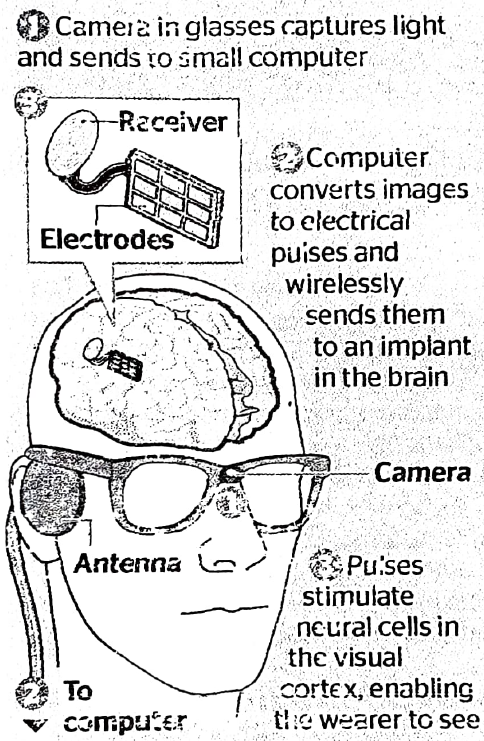
\includegraphics[width=\columnwidth]{./images/image.png}

  \noindent
  Vogt-Koyanagi-Harada syndrome, had an array of electrodes inserted into the
  back of her brain. An antenna was also connected through a hole in her skull.

  Doctors then sent signals to it, and she reported seeing them. They are now
  awaiting permission to connect it directly to a camera in the hope that they
  can retrain the woman's brain to recognise visual stimuli. Even though they
  have not yet performed this crucial final step, they said they were cautiously
  pleased with the progress so far.

  \columnbreak

  \enquote{This initial success in a patient is an exciting and important
  milestone even though it does not yet include a camera}, said Dr Greenberg.
  \enquote{Bypassing the optic nerve and directly stimulating the visual cortex,
  the Orion I has the potential to restore useful vision to patients completely
  blinded due to virtually any reason, including glaucoma, cancer, diabetic
  retinopathy, or trauma. Today these individuals have no available therapy and
  the Orion I offers hope, increasing independence and improved quality of
  life.}

  At the moment no one is pretending that the system will produce anything
  approaching normal sight. Nevertheless, the work in Manchester has shown that
  even the restoration of modest amounts of vision can significantly improve
  people's lives.

  Earlier this year Rhian Lewis, 49, spoke about receiving a bionic eye that
  worked using a retinal implant. Although it had nowhere near the resolution
  required to allow her to read or perform tasks that most take for granted, she
  described it as \enquote{like Christmas Day}. \enquote{Within seconds, there
  was this flashing in my eye, which has seen nothing for over 16 years, so it
  was like, oh my God, wow!} she said. \enquote{When I locate something,
  especially like a spoon or a fork on the table, it's pure elation. I get so
  excited.}

  Dan Pescod, of the Royal National Institute of Blind People, said the research
  was at an early stage, but added: \enquote{This is a very exciting and
  potentially life-changing development.}
\end{multicols}
\end{document}
